\section{Relating new information to the pangenome}

\subsection{Visualization}
% Adam
% Simon
% Josiah


Visualization of pangenome graphs presents novel challenges, because their data structure is complex, multidimensional, and nonlinear.
Traditional genome browsers neatly organize into a 2D rectangular shape, with 1D linear sequence on the x-axis and annotations on the y-axis.
In contrast, graph genomes follow network topology which requires three dimensions to render without overlapping lines.
Annotation tracks add another dimension, forcing all graph visualizations to involve some degree of flattening.  
Genome graph visualization tools can be considered in terms of their target applications. 
Many tools support the interpretation of assembly graphs. 
These tend to focus on the overall structure of the graph. 
In contrast, tools designed to support pangenome graph (often variation graph) visualization must additionally describe the relationship between genomes and the graph in which they are embedded.
An overview of tools features is given in Table \ref{table:Visualization_Features}.
\begin{table}[h!]
\hyphenation{nucleotide complexity}
\centering
\caption{An overview of graph visualization tools. \textbf{app:} application. \textbf{cli:} command line.}
\vspace{10mm}
\label{table:Visualization_Features}
\begin{tabular}{|p{2.5cm}|p{1.5cm}|p{2cm}|p{2.5cm}|p{2cm}|} 
 \hline
 \textbf{Tool} & \textbf{Layout Paradigm} & \textbf{Target Use Case} & \textbf{Scale of Data} & \textbf{Technical Notes} \\
 \hline
 \hline
Bandage & \multirow[c]{11}{=}{force-directed} & assembly graphs & 100 megabase variation graph, no nucleotide level & interactive desktop app \\ \cline{1-1} \cline{3-5}
GfaViz &  & assembly graphs, variation graphs & \multirow{12}{=}{megabase subgraph of a variation graph, no nucleotide level} & interactive desktop app, GFA2 support, OGDF\cite{Chimani_2012_OGDF} \\ \cline{1-1} \cline{3-3} \cline{5-5}
SHIMMER Sketch Graph &  & variation graphs &  & cli app, static images, GraphViz, Gephi \\ \cline{1-3} \cline{5-5}
SGTK & \multirow{7}{=}{force-directed, genome browser mode} & scaffold graphs, assembly graphs, reads, reference sequences &  & interactive web app, cytoscape.js\cite{Franz_2016_cytoscape} \\ \cline{1-1} \cline{3-5}
AGB &  & assembly graphs, reference sequences & topological complexity: thousands of edges\footnote{\url{https://github.com/almiheenko/almiheenko.github.io/blob/8f4b2f8c7c498f04fa32f53f69b4bc59888a14f0/AGB/Flye_Human/data/repeat_graph.json}} & interactive web app, d3-graphviz\footnote{\url{https://github.com/magjac/d3-graphviz}} \\\hline
SequenceTubeMap & pseudo-linear tubemap & \multirow{18}{=}{variation graphs} & from nucleotides to kilobases & interactive web app, unique layout \\ \cline{1-2} \cline{4-5}
MoMI-G & pseudo-linear tubemap, circos, linear annotation &  & gigabase circos, from nucleotides to kilobases & interactive web app, multiple views \\ \cline{1-2} \cline{4-5}
vg view & force-directed &  & 10 kilobase subgraph of a variation graph, nucleotide resolution & cli app, static image, GraphViz\\ \cline{1-2} \cline{4-5}
vg viz & \multirow{7}{=}{rectangular sorted matrix} &  & 100 kilobase subgraph of a variation graph & cli app, static image \\ \cline{1-1} \cline{4-5}
odgi viz &  &  & from nucleotide resolution to gigabase genomes & cli app, static image, binning \\\hline
\end{tabular}
\end{table}

Bandage \cite{Wick_2015}, GfaViz \cite{Gonnella_2018}, SGTK \cite{Kunyavskaya_2018} and AGB \cite{Mikheenko_2019} were designed to explore assembly graphs.
Bandage is the oldest and most widely used, supporting a wide range of formats and graph  paradigms, however it does not currently support GFA2 \citep{Mikheenko_2019}.
Force-directed graph layouts present an aesthetically pleasing way to layout a graph but it can be challenging to understand annotation woven through a 2D layout.
For this reason, SGTK and AGB offer a more traditional genome browser mode as well.
Except for GfaViz, they do not have the ability to structure the display using known linearization information. 

When choosing a tool, one also must consider the advantages of web applications versus local computation.  
Web apps have the option to serve precomputed content to any user, lowering end-user system requirements.
Local applications can benefit from institution specific resources including HPC and private data (see Table \ref{table:Visualization_Features} Technical Notes).

For variation graphs, SequenceTubemap \cite{Beyer_2019} displays regions using a visual language inspired by transit system maps.
This tool is useful for visualizing precise base-scale variation and short read mapping locations in human-chromosome-scale graphs.
However, its limited graph simplification tools make it difficult to use on larger regions.

There is a difference in scale when moving from an assembly or scaffold graph to a comprehensive variation graph of a species pangenome.
While tools like SGTK and AGB have been demonstrated on graphs with tens of thousands of entities, the 1000 Genomes Project dataset contains 88 million known human variants \citep{1000_2015}, which gives a density over the 3 billion base human genome of about 34 bases per variant, and a comprehensive variation graph with tens to hundreds of millions of elements---a much larger graph than those that SGTK and AGB have been shown to work with.
Moreover, to achieve visualization output file sizes on the scale of megabytes given hundred megabase- to gigabase-scale assemblies, these tools necessarily hide sequence information.

%Bandage currently only supports GFA1. GfaViz has full support for newer GFA2 features, such as gaps for representing scaffold graphs in addition to assembly graphs \citep{Gonnella_2018}.

%Two recent graph visualization tools, \texttt{SGTK} and \texttt{AGB}, are web applications in which the visualization is precomputed, lowering end-user system requirements \citep{Kunyavskaya_2018,Mikheenko_2019}.
%SGTK is designed for visualizing scaffold graphs, which can have negative-overlap gaps between sequenced segments, and is based around the in-browser Cytoscape.js graph layout library \citep{Kunyavskaya_2018}.
%It includes a potentially highly interpretable, ``browser'' layout structured around a reference sequence.  
%Though its presentation is less purpose built than the bands of Bandage.

%AGB has a similar overall design to SGTK, but makes different implementation choices.
%It is relatively tightly tied to the assembly graph use case, requiring each (sequence-bearing) edge to be classifiable as ``unique'' or ``repetitive'' based on assembler annotation or sequencing coverage \citep{Mikheenko_2019}.
%AGB is built around the idea of splitting up an assembly graph and visualizing portions of it, and features many ways to do this, including linear reference based and minimum edge cut based approaches.

MoMI-G is a multi-scale genome graph browser currently under development \cite{yokoyama_momi-g:_2019}. It employs SequenceTubemap at nucleotide scale and integrates it into a  framework along side a Circos \cite{Krzywinski_2009_Circos} plot for chromosome scale connections. 
The integration of multiple visualizations brings their strengths to bear on different areas. 
MoMI-G is currently the only tool that can visualize long reads to show structural variants against multiple haplotypes in a graph genome.

\texttt{vg viz} can render graphs of arbitrary size and complexity in linear time by sorting the sequence-bearing nodes of the graph into a one-dimensional layout \citep{Garrison_2019}. 
The tool is designed around a base-level visual representation of the graph, and optimized for comparing long embedded paths in the graph, on the basis of which nodes they do or do not visit. 
It can be difficult to understand high level or nonlinear structures in such a linearized layout. 
\texttt{ODGI viz}\footnote{\url{https://github.com/vgteam/odgi}} uses a layout very similar to \texttt{vg viz} and addresses scalability by binning hundreds of adjacent nodes together, thus reducing the resolution and making it possible to render the overall structure of gigabase pangenomes in a single image.

Figure~\ref{fig:visualization} provides a visual overview of the visualization methods surveyed here.
It remains an open problem to interactively visualize a comprehensive human pangenome graph, potentially including interchromosomal connections, at a variety of zoom levels to enable precision pangenomics at any scale.

\begin{figure}[h]
    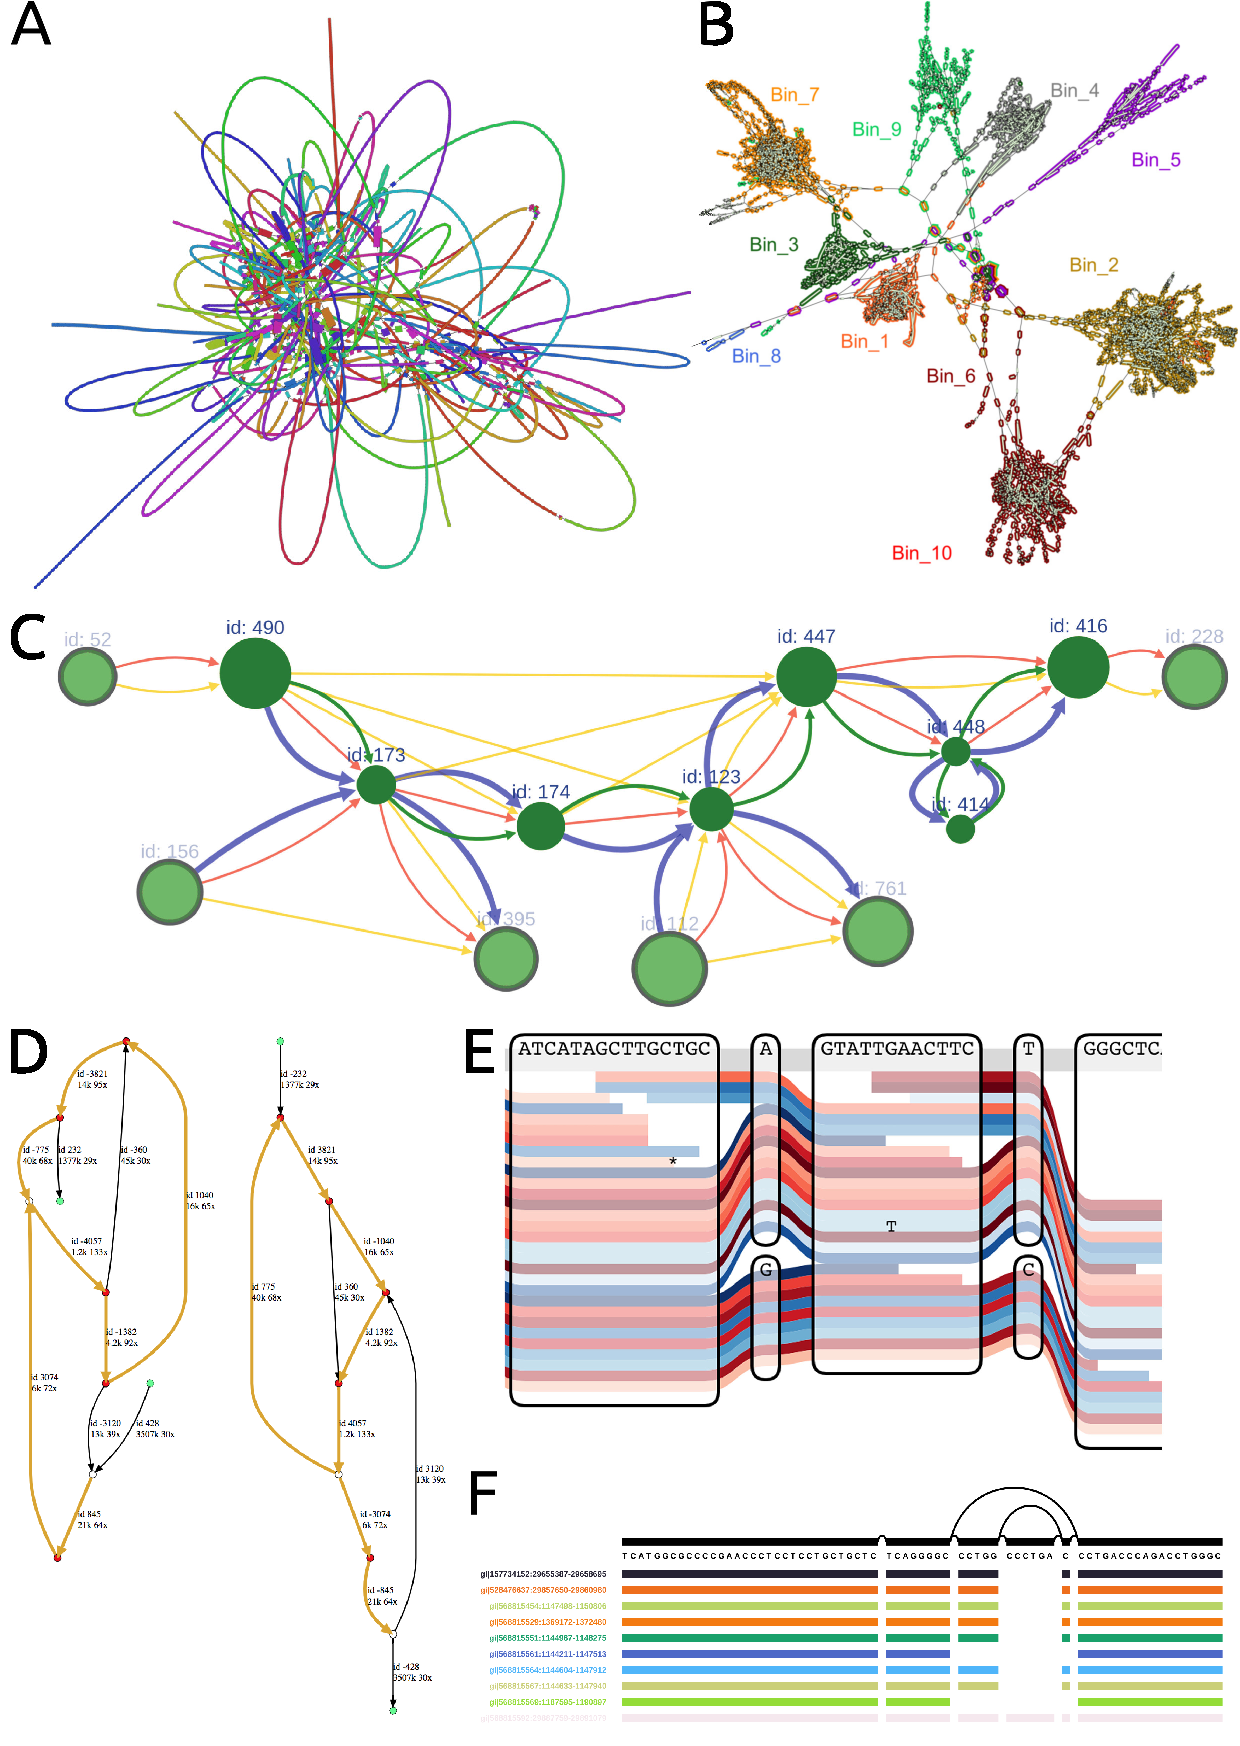
\includegraphics[width=0.9\textwidth]{figures/visualization.pdf}
    \caption{\label{fig:visualization} An overview of several approaches to visualizing assembly, scaffold, and comprehensive pangenome graphs.
\textbf{A:} Bandage, adapted from \cite{Wick_2015} supplementary section~6.
\textbf{B:} GfaViz, adapted from \cite{Gonnella_2018} supplementary figure~S4.
\textbf{C:} SGTK, adapted from \cite{Kunyavskaya_2018} figure~1.
\textbf{D:} AGB, adapted from \cite{Mikheenko_2019} supplementary figure~S3.
\textbf{E:} Sequence Tube Map, adapted from \cite{Beyer_2019} figure~2.
\textbf{F:} \texttt{vg viz}, adapted from \cite{Garrison_2019} figure~2.20.}
\end{figure}


%\citep{Wick_2015} : Bandage
%\citep{Gonnella_2018} : GfaViz
%\citep{Kunyavskaya_2018} : SGTK
%\citep{Mikheenko_2019} : AGB
%\citep{Beyer_2019} : TubeMap
%\citep{Garrison_2019} : Thesis

% JME: This section has been moved to the introduction

%\subsection{Finding structures in pangenome graphs}
%% Jordan
%
%\todo[inline]{JME: We need to decide whether to do this section}

\subsection{Graph alignment algorithms}

As noted above, genomic sequence data often can only be interpreted in the context of other sequences. 
For this reason, sequence comparison is at the core of many genomic analyses, and sequence alignment is the essential method for doing so. 
However, classic alignment algorithms like Smith-Waterman \cite{Smith_1981} do not directly apply to genome graphs, which comprise the majority of pangenomic models. 
Accordingly, the increasing prominence of genome graph methods has been enabled by fundamental algorithmic research in graph alignment, and it has also spurred further research.

The trend in the graph alignment research is toward greater generality and faster run time. 
The generality comes in two main forms. 
First, algorithms apply to increasingly general classes of graphs. 
The first widely-used algorithm for aligning biological sequences to graphs, partial order alignment, applied only to graphs without cycles \cite{Lee_2002, Grasso_2004}. 
More recent research has described algorithms that align to graphs with any shape \cite{Antipov_2015, Rautiainen_2017, Jain_2019a}. 
Second, graph alignment researchers have developed algorithms that use increasingly general scoring functions. 
Some earlier algorithms require restricted scoring functions to achieve efficiency \cite{Rautiainen_2017}, but recent contributions have used the less restricted scoring functions that are required to produce biologically meaningful alignments in many contexts \cite{Jain_2019a}.

Graph alignment research also has improved the algorithms' run time. 
Partial order alignment required acyclic graphs in order to run at comparable speed to linear sequence alignment algorithms \cite{Lee_2002}. 
Later optimizations simply ran slower on general graphs \cite{Kavya_2019}.
It has now been shown that graph alignment can run at the same asymptotic speed as linear alignment \cite{Jain_2019a}.
Further, there is a strong argument that this speed is essentially optimal \cite{Equi_2019}. 
In fact, these results were already known in other fields.
Many of the recent advances in graph alignment came from rediscovering analogs to the graph alignment problem in the related areas of regular expressions and hypertext \cite{Myers_1989, Amir_1997, Navarro_2000}. % hein1989new, ?
In addition to these theoretical results, researchers have also developed modified algorithms that run quickly the practical context of real-world computer architectures \cite{Suzuki_2018, Rautiainen_2019, Jain_2019b}.

%From a practical standpoint, the primary benefit of the research in alignment algorithms has been in aiding the design of read mapping tools. 
%Graph alignment algorithms are a central component of the graph mapping tools described below.

\subsection{Genome graph mapping}

Once a significant barrier to pangenomics research, the field now provides an array of well-performing, increasingly efficient read mapping tools for genome graphs. 
In some ways, the current landscape resembles the early days of short reads mappers for conventional references. 
A diversity of tools are now available, each experimenting with different algorithmic ideas. 
However, the field has not yet coalesced around any standard tool in the way conventional mapping now has around BWA-MEM \cite{Li_2013}. 

To the extent that a standard exists, it is currently VG \cite{Garrison_2018}---at least in the sense that later tools have largely chosen it as a point of comparison for their own performance \cite{Guo_2018,Kim_2019,Vaddadi_2019,Rautiainen_2019b}. 
It remains to be seen if VG will retain this position, or if another tool will emerge as the standard, or if a diversity of tools will be continue to be used. 
The ideal situation is probably the latter. 
The available tools represent a menu of tradeoffs that could be matched to different studies' unique requirements.

Invariably, genome graphs mappers make use of the seed-and-extend paradigm that has also been successful for linear references.
This methodology consists of first indexing the reference for exact match queries.
Then, the index is queried with a sequencing read for exact match ``seeds'', which are used to narrow in on small regions of the reference.
Expensive approximate-match alignment algorithms can then be targeted at these smaller regions to ``extend'' the seeds into full alignments. 
As this description suggests, a mapping tool's features are in large part determined by its choice of an indexing method and an alignment algorithm.
Genome graph indexing and alignment have both been active areas of research, as discussed above.
In addition, some tools employ an additional step to cluster seeds by their position on the graph before aligning.
While common for conventional mappers, the clustering step has proven challenging in genome graphs, and some tools omit it entirely.



%exhaustive traversals: debga-vara, 7 bridges

% general themes
%-need to control memory
%-need to employ approximate alignments
%-improved performance mapping to variants and calling variants from mappings
%-historically, divided into variation graph mapper

%IDEA: first commonalities, then differences



One major point of distinction between mapping tools is the type of graphs they were designed for. 
Several tools apply only to acyclic variation graphs, often the largely linear graphs that are formed by adding substitution and indel variants to a linear reference.
Examples include GenomeMapper (an early forerunner) \cite{Schneeberger_2009}, Seven Bridge's Graph Genome Aligner \cite{Rakocevic_2019}, HISAT2 \cite{Kim_2019}, V-MAP \cite{Vaddadi_2019}.
Another set of tools focus on de Bruijn graphs: BGREAT \cite{Limasset_2016}, deBGA \cite{Liu_2016}, and BrownieAligner \cite{Heydari_2018}.
Most of these were developed in parallel to recent pangenomics research, often with motivations in genome assembly. 
VG \cite{Garrison_2019} and GraphAligner \cite{Rautiainen_2019b} appear to be the only tools with open ambitions of mapping to arbitrary variation graphs, including complex local and global topologies encoding all kinds of variation.
GraphAligner is notable in that it can also align to generic overlap graphs.

The majority of these tools emphasize mapping short-read \emph{next-generation sequencing (NGS)} data. 
%Most likely, the motivation for doing so is the same as why NGS remains the standard for conventional resequencing experiments; the price point currently favors it. 
%In this sense, pangenomic graph mappers essentially represent an incremental technical improvement over previous pipelines, albeit a very important one. 
To our knowledge, GraphAligner and V-MAP are the only graph mapping tools that explicitly targets high-error long read sequencing data \cite{Rautiainen_2019b, Vaddadi_2019}, although others are in development \cite{Li_2019}.
V-MAP is also demonstrated on NGS reads, but GraphAligner's seeding strategy limits it to of long reads

% a paragraph about the approximations used?

Among the graph mappers that emphasize variation graphs, a theme has emerged about their accuracy. 
They typically do not improve mapping accuracy over the entire genome compared to state-of-the-art linear mappers. 
However, they do significantly improve read mapping accuracy \emph{over variants} \cite{Garrison_2019, Rakocevic_2019, Kim_2019}. 
In this, we see a concrete example of pangenomic methods mitigating reference bias. 
The unimproved (and often slightly diminished) performance over the rest of the genome probably indicates a combination of the relative nascency of the graph mapping tools and the burden of more complicated computational heuristics.

The actual algorithms that each tool employs vary greatly. 
For indexing, most graph mapping tools have opted for some variation of a $k$-mer table. 
In the case of de Bruijn graph mappers, this is an especially attractive option since the $k$-mers also implicitly define the edges of the graph. 
This may be why all of the de Bruijn graph mappers listed above use this strategy \cite{Holley_2012, Limasset_2016, Liu_2016, Heydari_2018, Rautiainen_2019b}. 
Additionally, GenomeMapper, Seven Bridge's mapper, and V-MAP seed with $k$-mer tables \cite{Schneeberger_2009, Rakocevic_2019, Vaddadi_2019}. 
The remaining mappers use succinct text indexes.
VG uses the GCSA2 \cite{Siren_2017} and a longest-common-prefix array, which enable very specific maximal-exact-match queries.
The cost is that the index is large, which contributes to VG's high memory utilization \cite{Garrison_2019}.
HISAT2 uses a modified GCSA \cite{Siren_2014}  that also encodes the graph structure itself.
This helps give HISAT2 an impressively low memory footprint at the expense of a somewhat more limited set of queries \cite{Kim_2019}.
GraphAligner uses either minimizer or full text indexes of the node sequences of the graph, but the memory savings of these are offset by large in-memory structures that it uses to support its efficient alignment algorithm, yielding runtime memory costs similar to those of VG \cite{Rautiainen_2019b}.

Most de Bruijn graph mappers have used searches through the graph to make alignments.
deBGA exhaustively enumerates paths, but it reduces the potentially exponential space of sequences to align to with a clustering step.
Its core alignment algorithm is actually a sequence-to-sequence algorithm applied to each path \cite{Liu_2016}.
BGREAT addresses the combinatorial complexity of the extension step by greedily choosing a path in the graph.
This is fast, but provides no optimality guarantees, and their algorithm does not support indels \cite{Limasset_2016}.
Unfortunately, neither deBGA nor BGREAT compare their performance to any graph-based tools, and the somewhat unnatural context for the linear mappers they compare to makes their evaluations hard to interpret.
BrownieAligner also exhaustively explores paths out from a seed, but it uses a branch-and-bound algorithm to prune the search space along the way.
%It also has a unique trick of choosing paths partially based on a Markov model trained on the reads.
%This is essentially a limited form of read-backed phasing.
According to the authors' analysis, BrownieAligner is more accurate than deBGA and BGREAT, but BGREAT tends to be more memory efficient, and deBGA tends to be faster \cite{Heydari_2018}.
Finally, GraphAligner is the only de Bruijn graph mapper to take advantage of recent research into graph alignment algorithms.
It uses a banded alignment algorithm to achieve impressive speed aligning long reads to genome graphs, requiring around twice the runtime of minimap2 \cite{Rautiainen_2019b, Li_2018}.

While few of the de Bruijn graph mappers employ graph-based alignment algorithms, most variation graph mappers do. 
One exception is GenomeMapper, which aligns to all paths out from a seed. 
However, GenomeMapper also seems to be unmaintained since 2009, and it has heuristics that are better suited to earlier NGS technologies \cite{Schneeberger_2009}. 
Seven Bridges' mapper, VG, and V-MAP all employ some version of partial order alignment \cite{Rakocevic_2019, Garrison_2019, Vaddadi_2019}. 
Seven Bridges also tries to find a near-match using a potentially exponential depth-first search algorithm before resorting to alignment algorithms that are more expensive when variation is sparse \cite{Rakocevic_2019}. 
The HISAT2 alignment algorithm is a complex set of heuristics that lean heavily on the exact match queries from its optimized index. 
This makes it exceptionally fast, although it also can hurt alignment quality around indels. 
In general, VG compares favorably to other tools in terms of accuracy on NGS data. However, most comparisons point out that it is quite demanding on computer memory and often slower than the alternatives \cite{Kim_2019, Vaddadi_2019}. 
V-MAP uses distance-based heuristics on acyclic graphs to efficiently cluster seeds. 
This allows it to align high-error long reads more efficiently than VG, although to our knowledge there has yet to be a published comparison to GraphAligner \cite{Vaddadi_2019}.


\begin{table}[h!]
\centering
\caption{An overview of graph mapping tools}
\vspace{10mm}
\label{table:mappers}
\begin{tabular}{|p{2.25cm}|p{2.5cm}|p{1.75cm}|p{2.5cm}|}
 \hline
 \textbf{Tool} & \textbf{Graph Types} & \textbf{Sequencing Types} & \textbf{Other Notes} \\
 \hline
 \hline
deBGA & \multirow[c]{3}{=}{De Bruijn graph} & \multirow[c]{3}{=}{NGS} &  \\ \cline{1-1} \cline{4-4}
BGREAT &  &  & Gapless alignment  \\ \cline{1-1} \cline{4-4}
BrownieAligner &  &  &   \\ \hline
GenomeMapper & \multirow[c]{4}{=}{Acyclic variation graph} & \multirow[c]{3}{=}{NGS} & No longer maintained \\ \cline{1-1} \cline{4-4}
Graph Genome Aligner &  &  &  \\ \cline{1-1} \cline{4-4}
HISAT2 &  &  & Fast \\ \cline{1-1} \cline{3-4}
V-MAP &  & NGS and long read & \\ \hline
VG & Variation graph & NGS and long read & Accurate, high memory usage \\ \hline
GraphAligner & Variation graph or overlap graph & Long read & Fast \\ \hline
%GfaViz &  & assembly graphs, variation graphs & \multirow{15}{=}{megabase subgraph of a variation graph, no nucleotide level} & interactive desktop app, GFA2 support, OGDF\cite{Chimani_2012_OGDF} \\ \cline{1-1} \cline{3-3} \cline{5-5}
%SHIMMER Sketch Graph &  & variation graphs &  & cli app, static images, GraphViz, Gephi \\ \cline{1-3} \cline{5-5}
%SGTK & \multirow{10}{=}{force-directed, genome browser mode} & scaffold graphs, assembly graphs, reads, reference sequences &  & interactive web app, cytoscape.js\cite{Franz_2016_cytoscape} \\ \cline{1-1} \cline{3-5}
%AGB &  & assembly graphs, reference sequences & topological complexity: thousands of edges\footnote{\url{https://github.com/almiheenko/almiheenko.github.io/blob/8f4b2f8c7c498f04fa32f53f69b4bc59888a14f0/AGB/Flye_Human/data/repeat_graph.json}} & interactive web app, d3-graphviz\footnote{\url{https://github.com/magjac/d3-graphviz}} \\\hline
%SequenceTubeMap & pseudo-linear tubemap & \multirow{23}{=}{variation graphs} & from nucleotides to kilobases & interactive web app, unique layout \\ \cline{1-2} \cline{4-5}
%MoMI-G & pseudo-linear tubemap, circos, linear annotation &  & gigabase circos, from nucleotides to kilobases & interactive web app, multiple views \\ \cline{1-2} \cline{4-5}
%vg view & force-directed &  & 10 kilobase subgraph of a variation graph, nucleotide resolution & cli app, static image, GraphViz\\ \cline{1-2} \cline{4-5}
%vg viz & \multirow{7}{=}{rectangular sorted matrix} &  & 100 kilobase subgraph of a variation graph & cli app, static image \\ \cline{1-1} \cline{4-5}
%odgi viz &  &  & from nucleotide resolution to gigabase genomes & cli app, static image, binning \\\hline
\end{tabular}
\end{table}

%\todo{JME: why are we going into so much detail about HISAT2 compared to the other tools?}
%HISAT2 is a BWT-based mapping algorithm that uses an adaptation of the Ferragina-Manzini (FM) index, a hierarchical graph FM index (HGFM).
%\todo{JME: it actually uses a GCSA, not a standard FM index}
%An FM index is a compressed representation of the graph that is optimized for substring searching.
%The HGFM is comprised of two FM indexes: a global index of the entire genome and local indexes of smaller portions of the genome and their variants.
%Repeat sequences are combined into a separate index, keeping only one copy of each repeat so sequences in repetitive regions are only aligned once.
%Alignment is done by searching the FM indexes, starting with the global index.
%
%
%Each of these graph alignment tools has demonstrated an increase in sensitivity over mapping to a standard linear reference.
%\todo{JME: what tools are you referring to with "each"? you've only referred to one tool}
%GenomeMapper, vg map, Seven Bridges' mapping algorithm, and HISAT2 are primarily short read mappers.
%\todo{JME: i think 7bg's tool is called Graph Genome Aligner}
%GraphAligner is a long read mapper and V-MAP is used for both.
%V-MAP doesn't align reads itself but finds a small subgraph that a read can be aligned to using existing mappers. 
%HISAT2 and vg can align both RNA and DNA.


%VMAP
%-only for DAGs
%-minimizer of most paths for index
%-linear embedding based on distance from source node for clustering
%-finds better mappings than vg for short reads, worse for long reads
%-significantly faster than map in their evaluations
%-uses GSSW for alignment

%GraphAligner
%-focus on long reads aligned to de bruijn graphs
%-does not chain seeds
%-indexes minimizers on only  node sequences, not paths
%-uses banded version of bit-parallel algorithm with tweaks
%-banding is based on x-drop rather than classic parallelogram shapes
%-hard caps on amount of dp and priority queue in tangled regions
%-actually suitable for arbitrary graphs, i think
%-very fast for what it does

%7bg
%-referred to as Genome Graph Pipeline and Graph Aligner
%-k mer hash table along all paths, but with cap on total number of edges, thinned
%-employs clustering, but sketchy on details
%-multi-stage alignment:
%	-first gapless alignment with graph-aware BITAP algorithm
%	-GSSW if there are novel indels
%-only supports VCF DAGs
%-better precision and recall compared to bwa on reads with variants

%genomemapper
%-presented as a technique for mapping to species with high polymorphism
%-discuss reference bias
%-hash based indexing - short k-mers (5 to 13)
%-memory mapped index
%-does not use vcf, seems to use IUPAC for snps
%-some effort toward making a bit-efficient encoding
%-3 stage alignment
%	-find exact matches with k-mers
%	-extend to nearly-identical matches
%	-banded alignment if this fails
%-I don't get how the alignment handles the branching of the graph...
%	-oh, it seems this seeding step only applies to blocks, then tree unrolling
%-for some reason does intra-read task parallelism for tree unrolling
%-demonstrate advantages for indel calling and alignment

%hisat2
%-VCF style graphs, insertions limited to 20 bp
%-GFM representation, based on Jouni's prefix-sorted graphs
%-hierarchical index
%	-one global index with reference and many variants
%	-thousands of 50kb local indexes, partially overlapping
%	-in hisat1 paper, local indexes are presented as a way to find smaller matches in local regions near splice sites
%-50-60% slower with 14M variants that itself without variants
%-obtains greater accuracy on reads containing variants
%-low memory usage: 6.2 GB (self-indexed)
%-compress repeat sequences in the genome and align to them with BWT-FM index
%	-identified by a k-mer count of 100-mers
%	-construct a de bruijn graph of frequent k-mers and then do greedy walks in it to identify sequences
%-i wonder if the reason they need to do this business with the repeats is that the strategy of finding a fixed number of exact matches and relying on pidgeonhole principle performs poorly against the repeat content of the non-coding genome
%	-do they actually do this method? the hisat supplement describes a pretty complicated set of heuristics

%debga-vara
%-emphasizes RAM usage
%-uses landau-vishkin algorithm (fast approximate algorithm with < k edits)
%	-banded, edit distance penalty
%-seem to emphasize low memory footprint
%-possibly doing tree unrolling? or maybe aligning to a suffix tree?
%	-sounds to me like tree unrolling with skips for indels
%-seems to only index the reference, not any variation
%-claims faster speed that BWA-MEM and better performance
%-the results they get on certain tools make me question the whole evaluation
%-i get the sense that when they say a problem is NP-hard, they actually mean that they wrote an exponential algorithm for it

%minigraph
%-does not yet give base-level alignment
%-intended for coarse graph without too much small variation
%-minimizer hash table for seeding
%-linear chains on nodes, followed by multi-path distance search between chains
%-

%make a section about controlling memory usage? -- emphasis of debga vara and hisat2

%gaffe?

%ggmap/bgreat - greedy matching from each overlap seed, align to entire unitigs at a time
%-start a new mapping for each "first seed"
%-find that blastgraph has serious scalability problems

%it seems all of the DBG methods use some kind of DFS type search (possibly greedy or BnB)

%liu-debga
%-index all kmers of unitigsg


%\subsection{De Bruijn graph mappers}
%% Adam
%
%% Style Note: apparently de Bruijn Graph should be lower case unless otherwise required to be capitalized.
%
%In addition to mappers designed to map to general graphs, a selection of mappers designed to map specifically to de Bruijn graphs, or to compacted de Bruijn graphs\todo{Did we define this already?}, have also been developed.
%
%One of the first of these, BlastGraph from 2012, uses an edit distance alignment metric for scoring, and finds all matches in the graph within that edit distance \citep{Holley_2012}.
%However, it seems better suited to search than to mapping to support resequencing; but it is only shown running on up to 10,000~reads at a time \citep{Holley_2012}.
%The actual alignment algorithm uses a hash-table-based seed index combined with a recursive-depth-first-search-based extension step, and is shown applied to de Bruijn graphs and ordinary sequence graphs \citep{Holley_2012}.
%\todo{Can we move this to the previous section since it doesn't really do anything de-Bruijn-specific?}
%
%\citeauthor{Holley_2012} do not discuss the algorithmics of their alignment approach, beyond demonstrating that it is sufficiently fast in practice \citep{Holley_2012}.
%In \cite{Limasset_2016}, \citeauthor{Limasset_2016} present a proof that the ``de Bruijn Graph Read Mapping Problem'' (when looking for acyclic mappings) is NP-complete, by a reduction of the Hamiltonian Path Problem, through a Traveling Salesman Problem variant, and then through a gapless, acyclic read-to-sequence-graph mapping problem \citep{Limasset_2016}.
%This realization of NP-completeness goes on to structure future work in the field.
%See also, however, the Dijkstra's-algorithm-based polynomial-time solution given in \cite{Antipov_2015} to the problem of finding the optimal path between a particular anchoring source and sink.
%
%\citeauthor{Limasset_2016} present a greedy tool, BGREAT, which avoids the theoretically exponential recursive-depth-first-search step of BlastGraph, and which leverages the overlaps between nodes in the compacted de Bruijn graph as seeds \citep{Limasset_2016}.
%This seed selection mechanism inherently limits the number of seed hits which need to be indexed, and provides (modulo errors) some intuitive guarantees about the distribution of seeds in a true mapping \citep{Limasset_2016}.
%However, the authors compare BGREAT only against Bowtie2, and it is unclear how to interpret their comparison results, as Bowtie2 is, with BGREAT, part of their larget GGMAP, and moreover does not align to graphs \citep{Limasset_2016}.
%
%While BGREAT is motivated in terms of mapping to assembly graphs \citep{Limasset_2016}, the deBGA tool, also published in 2016, is aimed at mapping to ``Reference de Bruijn Graphs'' describing variation within or between species \citep{Liu_2016}.
%The mapping algorithm uses the $k$-mers of the de Bruijn graph as seeds, and unlike BGREAT and BlastGraph the core alignment operation is sequence-to-sequence \citep{Liu_2016}.
%Also unlike BGREAT and BlastGraph, however, deBGA provides a paired-end mapper \citep{Liu_2016}.
%Speed and accuracy compare favorably with linear-reference-based tools, but again no comparison against other graph-based tools is made \citep{Liu_2016}.
%\todo{The BrownieAligner paper accuses BGREAT of not supporting indels; BGREAT says it allows an ``edit or Hamming distance'', which is ambiguous between supporting both or characterizing edit distance as just meaning Hamming distance.}
%
%A more recent read to graph mapping tool, 2018's BrownieAligner, is compared against both BGREAT and deBGA; although it can be slower, it is more accurate, because it is able to compute genuinely optimal alignments in reasonable time \citep{Heydari_2018}.
%It accomplishes this by using a branch-and-bound approach to limit its depth-first search out from each de Bruijn $k$-mer or fallback MEM seed \citep{Heydari_2018}.
%Additionally, BrownieAligner allows a ``higher-order Markov model'', specifying the probability of each de Bruijn graph node as a function of the previous $n$-node path taken through the graph, to constrain the possible paths through the graph against which reads are aligned \citep{Heydari_2018}.
%This is similar to the idea behind using haplotypes to inform mapping in sequence graphs \citep{Siren_2019}, except that in BrownieAligner the Markov model describing acceptable paths is learned from a first pass of read alignment, after which the sufficiently-covered paths in the graph become the paths in the Markov model used to restrict a second alignment pass \citep{Heydari_2018}.
%In this way, some variant- or sample-level information can be extracted from the read set as a whole and fed back into the individual read mappings, improving their accuracy \citep{Heydari_2018}.



% Useful to map to dBGs

% BlastGraph
    % Works on dBGs and other SGs
    % Find paths within edit distance of query
    % Hash table index of all seeds of a certain length
        % Stores only start positions
    % Compute edit distances and alignments out in both directions from each seed
        % Deduplicate when multiple seeds suggest the same alignment
    % Wrote a Java Cytoscape plugin and a C implementation

% BGREAT
    % Works on dBGs and actually maps
    % Justified in terms of mapping to assemblies
    % Mapping to dBGs is NP-complete even without gaps
        % How does this square with the edit distance algorithm's algorithmics?
            % Finding all the seed starts in the dBG for BlastGraph could be exponential for seeds longer than nodes
            % Recursive DFS tail edit distance alignment could also be exponential
            % But dBG overlap structure limits the density of braiding
        % The proof is by reducing Hmailtonian Path (path that visits each node once) -> restricted Traveling Salesman -> general graph mapping -> mapping to dBG
    % Actual tools: GGMAP (BGREAT + Bowtie2 for unitigs), and BGREAT for branching paths
        % BGREAT uses the dBG overlap regons themselves as seeds
        % They think they can get away with only mapping with Bowtie2 if they don't find a good mapping with BGREAT
            % They might be right; the dBG structure kind of precludes any competitive mappings in the middle of unitigs when there's a good mapping that covers an overlap
                % Because if there was another similar place in the genome it would have an overlap with the stuff it is similar to
        % Uses a greedy threading approach starting from the outer overlap sequences that occur in the read
            % Drop the whole read if it can't find a mapping for each end from the outermost overlap seeds.
        % Get linear time mapping which is nice
        % Not quite clear to me how they did the comparisons: are they just giving the time that their bowtie2 and blastgraph steps took on the reads that were fed to them?
            % Maybe they didn't find other comparable tools to compare to.

% deBGA
    % Justified in terms of mapping to variation and MSAs
    % "Putative Read Position" (PRP) (basically read start position/seed offset) 
    % Uses MEM-based seeding
    % Alignment is either exact match extension or aligning to "clustered" sequences, no string-to-graph
    % Paired end support (which BGREAT and BlastGraph don't mention)
    % Very fast, even on human
    % Not clear how reads are surjected to linear space for comparison
        % "Multiple equally best alignments"
            % deBGA and BWA with 1000 max mappings
        % If not surjected the problem is easier (no need to try to resolve repeats)

% hybridSPAdes
    % This is a short-and-long-read assembler, not a mapper
    % Maps long reads into a short-read dBG-derived graph
        % Just looks for 8 or more matching 13-mers to an "edge" for "support"
        % Does exponential string to graph alignment for the hard parts
        % Propose a polynomial algorithm for aligning between anchored ends for minimum edit distance

% BrownieAligner
    % Branch and bound approach to seed and extend
    % "Higher order markov model" to mark paths in the graph that exist, like our GBWT
        % Two pass approach where they train the markov model based on one batch of alignments and then realign
        % I think this is what lets them learn novel paths not in the linear reference but still catch errors
        % "Markov models offers a significant improvement for the alignment of these harder to align reads."
    % Lets seeds be smaller then dBG kmer size
    % "for each dataset the best accuracy for BrownieAligner is always higher than the best accuracy for other tools"

% Really comparing and contrasting the empirical speed, accuracy, etc claims of these tools would be hard and really requires independent experiments
    % Although BrownieAligner compares against BGREAT and deBGA
    

% BlastGraph (2012) \citep{Holley_2012}
% BGREAT (2016) \citep{Limasset_2016}
% deBGA (2016) \citep{Liu_2016}
    % deBGA-VARA is a variation-aware extension but not published open-access
% hybridSPAdes (2016) \citep{Antipov_2015}
% BrownieAligner (2018) \citep{Heydari_2018}

% See also: https://bmcbioinformatics.biomedcentral.com/articles/10.1186/s12859-016-1103-9

\subsection{Variation-aware transcriptomic mapping}

Attempts to use pangenomic models to analyze transcriptomic sequencing data have generally received less attention than similar methods with whole genome sequencing data.
However, certain downstream applications in transcriptomics also benefit from incorporating information on genomic variation.
Due to presence of splicing, mapping transcriptomic reads typically requires specialized algorithms.
Thus, variation-aware mappers for transcriptomic reads have largely been developed in parallel to mappers for genomic reads, although graphical methods have recently created some room for overlap.

Several methods have been published that specifically focus on reducing mapping bias for RNA-seq data around SNVs. 
GSNAP was the first such method \cite{Wu2010-hv}.
It seeds mappings with a hash table of $k$-mers from both the genome and a set of SNVs.
The current version uses a suffix array as well. 
ASElux, uses an individual's heterozygous exonic SNVs to create a suffix array index of the alleles and their flanking sequences \cite{Miao2018-ps}, which is used to filter reads that do not closely match some allele.
More expensive alignment algorithms are restricted to this smaller read set, which is all that is need for some transcriptomic applications.
Similarly to ASElux, iMapSplice creates an index of SNV alleles and their flanking sequences \cite{Liu_2018}.
The sequences are indexed using enhanced suffix arrays, and reads are mapped to both this index and the reference genome simultaneously.
The authors demonstrated that iMapSplice achieves higher mapping accuracy and lower reference bias compared to both a linear mapping method and HISAT2.
GSNAP is still competitive the later mapping methods with regards to mapping accuracy, but it is generally much slower \cite{Castel2015-ef}.
%Proper variant-aware mapping methods, on the other hand, do not require that the variants are phased beforehand.
%GSNAP was the first variant- and splicing-aware mapping method developed for RNA-seq data \cite{Wu2010-hv}. %\todo{JAS: We might want to add GSNAP introduction to the model section since it is general and also works for WGS}.
%It uses a $k$-mer-based approach where both the genome and a set of SNVs are indexed using hash tables.
%The current version uses a suffix array in addition to the hash table.
%GSNAP is still competitive contemporary mapping methods with regards to mapping accuracy, but it is generally much slower.
%Although not demonstrated in the initial publication, GSNAP does reduce reference bias around SNVs \cite{Castel2015-ef}.

%Another variant-aware method, ASElux, uses all heterozygous exonic SNVs in an individual to create a suffix array index of the alleles and their flanking sequences \cite{Miao2018-ps}. 
%This index is used to filter read pairs that does not overlap any SNVs with up to 2 mismatches. 
%The much smaller set of read pairs that pass this filter are then aligned to a different suffix array index consisting of exonic and intronic regions and pairs that align unique to a single gene are used for allele counting. 

%Similarly to ASElux, iMapSplice creates an index of SNV alleles and their flanking sequences \cite{Liu_2018}.
%The sequences are indexed using enhanced suffix arrays and reads are mapped to both this index and the reference genome simultaneously.
%The authors demonstrated that iMapSplice achieves higher mapping accuracy and lower reference bias compared to both a linear mapping method and HISAT2.

GSNAP, ASElux and iMapSplice only support SNVs and are therefore unable to reduce reference bias around indels.
In contrast, graph-based methods can easily model indels.
HISAT2 can map RNA-seq data in addition to genomic DNA \cite{Kim_2019}.
It is based on the RNA mapper HISAT \cite{Kim_2015}, and it retains the capacity for spliced alignment.
Otherwise, its mapping algorithm for transcriptomic sequencing is the same as for genomic DNA (See above).
Others have documented a reduction in mapping bias around SNVs for an early version of HISAT2 \cite{Liu_2018}. 
The ability to create spliced variation graphs has also been added to VG \cite{Garrison_2018}. 
In these variation graphs, known splice junctions are added as edges, similar to the addition of a deletion event.
VG supports any type of variation, but its splicing-awareness is limited to only known splice junctions.
Thus, reads that span a novel splice junction will only map partially.

%As with whole genome DNA sequencing data, variation-aware analysis of RNA-seq data is important for getting accurate results in highly polymorphic regions, such as the HLA genes in the human major histocompatibility complex region. 
%AltHapAlignR and HLApers have both demonstrated improvements in the estimation of HLA gene/transcript expression as a result of comparing the reads against a collection of known HLA haplotypes, instead of using the linear reference \cite{Lee_2018,Aguiar2019-fy}.


%\subsection{Non-graph population mapping tools}
% Erik

